\chapter{Itération 3}

Dans la dernière itération, nous avons collecté un grand ensemble de données
des différentes types. Malgré tout, ces données n'ont pas de valeur tel que on
ne les explore pas. C'est le rôle du Business Intelligence que nous allons
étudier dans cette itération.

\section{But de l'itération}

En accord avec le Product Owner, le but de cette itération est:

\begin{description}
    \item [Smartphone] L'ajout de nouvelles fonctionnalités comme:
        \begin{itemize}
            \item La détection des réseaux avec leur intensité.
            \item l'exploitation des données collectées selon les besoins.
        \end{itemize}
    \item [Rapport] Typage des rapports.
    \item [Dashboard] \textbf{}

        \begin{itemize}
            \item Élaboration des mécanismes d'authentification.
            \item Des nouveaux marqueurs qui spécifient chaque type de rapport
                ajouté.
        \end{itemize}
\end{description}

%Le Product Owner nous a demandé d'améliorer le chargement de l'image
%dans le serveur de telle sorte que la qualité d'image reste la même..
%Donc, dans cette itération, nous allons tenir compte des attentes du Product Owner. Nous allons
%modifier le critère de chargement, En plus nous allons implémenter une méthode
%permettant de maintenir la qualité.

\section{Planification de l'itération}

\subsection{Backlog de l'itération}

On définit dans le tableau~\ref{tab:sprint3-backlog} la liste de nos tâches
dans cette itération.

\begin{center}
    \footnotesize
    \begin{longtable}{| p{1cm} | p{5cm} | p{7cm} | l |}
        \caption{Tâches à faire de la troisième itération}
\label{tab:sprint3-backlog} \\

 \hline
 \multicolumn{1}{|c}{\textbf{Réf}} &
 \multicolumn{1}{|c}{\textbf{Spécification}} &
 \multicolumn{1}{|c}{\textbf{Description}} &
 \multicolumn{1}{|c|}{\textbf{P}} \\ \hline
 \endhead

 \hline \multicolumn{4}{|r|}{{Continué en page suivante$\dotsc$}} \\ \hline
 \endfoot

 \hline \hline
 \endlastfoot

\hline
3.1 & Intégration Dashboard et Rapport dans l'application Android & Implémenter la méthode qui affiche les pages ``Dashboard et Rapport'' chacun a un bouton spécifié   & 1 \\ \hline
3.2 & Authentification RESTful & Ajouter l'authentification dans le serveur pour assurer la sécurité & 1 \\ \hline
3.3 & Landing page & Créer une page Web pour la commercialisation et définition de \textquote{City Watch} & 3 \\ \hline
3.4 & Compte utilisateur & Modifications nécessaires pour le support des comptes d'utilisateur et l'intégration avec le reste des tableaux & 2 \\ \hline
3.5 & Service d'enregistrement les informations du réseau & Enregistrer les informations des réseaux cellulaires (opérateur, génération, force du signal) & 1 \\ \hline
3.6 & Service de récupération des informations réseaux  & Retourner les informations du réseaux cellulaire & 1 \\ \hline
3.7 & Service d'enregistrement de la vitesse du véhicule & Enregistrer les vitesses du véhicule le long de la trajectoire & 1 \\ \hline
3.8 & Service de récupération de la vitesse & Retourner la vitesse moyenne des véhicules dans une zone & 1 \\ \hline
3.9 & Application Android Responsive & Supporter plus résolutions & 3 \\ \hline
3.10 & Recherche Business intelligence & Utiliser le Business Intelligence et les solutions disponibles & 2 \\ \hline
3.11 & Intégrer la base de données avec BI & Intégrer BD du service web à la solution BI choisie & 2\\ \hline
3.12 & Logo du \textquote{City Watch} & Designer un Logo pour \textquote{City Watch} et pour ses applications & 3 \\ \hline
3.13 & Étude scénario de commercial d'embouteillage & Étudier les scénarios possibles pour le marketing des données d'embouteillage & 2\\ \hline
3.14 & Rectification du service de chargement d'image & Fixer les cas où l'image ne peut pas être chargée au serveur & 1 \\ \hline
3.15 & Étude scénario de commercial des secousses & Étudier les scénarios possibles pour le marketing des données de secousses & 2\\ \hline
% 3.16 & IHM & Ajout des boutons radio pour distinguer (pieton / voiture)(android) & 3 \\ \hline
\end{longtable}
\end{center}

%\begin{table}[H]
%    \centering
%    \begin{tabular}{| p{3cm} | l |}
%        \hline
%        Cas d'utilisateur & Authentification Utilisateur \\ \hline
%        Acteur & Utilisateur \\ \hline
%        Pré condition & Utilisateur non authentifié \\ \hline
%        Post condition & Utilisateur connecté \\ \hline
%        Description du scénario &
%        \begin{minipage}{11cm}
%            \vspace*{0.2cm}
%            \begin{itemize}
%                \item L'utilisateur ouvre la page Dashboard ou Rapport.
%                \item Le système affiche un dialogue d'authentification.
%                \item L'utilisateur saisit son émail et son mot de passe et clique sur le bouton ``Login''.
%                \item Le système envoie les informations d'identité au serveur.
%                \item Le serveur vérifie les information, retourne un jeton d'authentification.
%                \item Le système envoie le jeton d'authentification au serveur.
%                \item Le serveur vérifie le jeton d'authentification et retourne un jeton d'accès.
%                \item Le système affiche la cartographie et récupère les données à afficher.
%            \end{itemize}
%            \vspace*{0.2cm}
%        \end{minipage} \\ \hline
%        Exception & \begin{minipage}{11cm}
%            \vspace*{0.2cm}
%            \begin{itemize}
%                \item L'utilisateur n'a pas du compte.
%                \item Les informations d'identité sont invalides.
%            \end{itemize}
%            \vspace*{0.1cm}
%        \end{minipage}
%        \\ \hline
%    \end{tabular}
%    \caption{Description du cas d'utilisation ``Authentification Utilisateur''}
%\end{table}

\subsection{Estimation de l'itération}

Le tableau~\ref{tab:sprint3-capacity} représente le budget horaire des membres
dans les 3 semaines de l'itération.

\begin{table}[H]
    \centering
    \begin{tabular}{| c | c |}
\hline
\textbf{Membre} & \textbf{Budget Horaire} \\ \hline
\hline

Moez & 144\\ \hline
Rihab & 144 \\ \hline
\textbf{Total} & 288 \\ \hline
    \end{tabular}
    \caption{Budget Horaire --- Itération 3}
\label{tab:sprint3-capacity}
\end{table}

Le tableau~\ref{tab:sprint3-estimation} représente les estimations de nos tâches
en heures pour cette itération.

\begin{center}
    \begin{longtable}{| l | l | l |}
        \caption{Nombre d'heures estimé pour la réalisation des tâches}
\label{tab:sprint3-estimation} \\

 \hline
 \multicolumn{1}{|c}{\textbf{Spécification}} &
 \multicolumn{1}{|c}{\textbf{Membre}} &
 \multicolumn{1}{|c|}{\textbf{Heures}} \\ \hline
 \endhead

 \hline \multicolumn{3}{|r|}{{Continué en page suivante$\dotsc$}} \\ \hline
 \endfoot

 \hline \hline
 \endlastfoot

\hline
Intégration Dashboard et Rapport dans l'application Android & Rihab & 5 $\times$ 2 \\ \hline
Authentification RESTful & Rihab \& Moez & 13 $\times$ 2 \\ \hline
Landing page & Rihab & 13 \\ \hline
Compte utilisateur & Moez & 8 \\ \hline
Service d'enregistrement les informations du réseau & Moez & 5  \\ \hline
Service de récupération des informations réseaux  & Moez & 5  \\ \hline
Service d'enregistrement de la vitesse du véhicule & Rihab & 5  \\ \hline
Service de récupération de la vitesse & Rihab & 5  \\ \hline
Application Android Responsive & Rihab & 13 \\ \hline
Recherche Business intelligence & Moez & 13 $\times$ 2 \\ \hline
Intégrer la base de données avec BI & Moez & 13 $\times$ 2 \\ \hline
Logo du \textquote{City Watch} & Rihab & 13 \\ \hline
Étude scénario de commercial d'embouteillage & Rihab & 13 $\times$ 2 \\ \hline
Rectification du service de chargement d'image & Rihab & 13 $\times$ 2 \\ \hline
Étude scénario de commercial des secousses & Rihab & 13 $\times$ 2 \\ \hline
%IHM & Rihab & 5 $\times$ 2 \\ \hline
\end{longtable}
\end{center}

\section{Outils utilisés}

\subsection{OAuth2}

Pour sécuriser et limiter l'accès à nos services web, nous avons décidé
d'implémenter différentes technologies dont la première est
l'authentification.

Le choix naturel est OAuth2~\cite{RFC6749}. C'est un protocole de délégation
d'autorisation. Il permet aux applications \textquote{consommateurs} d'avoir la
permission d'utiliser un service web \textquote{fournisseur}.

\subsection{Business Intelligence}

La \acrfull{BI}\footnote{Informatique décisionnelle} propose d'utiliser les
données transitant par le système d'information en informations susceptibles
d'être exploitées à des fins décisionnelles.

Les 4 fonctions de la chaîne décisionnelle:

\begin{description}
    \item [\acrfull{ETL}] Collecter, nettoyer et consolider les données
        Extraire les données des systèmes de production et les adapter à un
        usage décisionnel.
    \item [\acrfull{DW}] Stocker Centraliser les données structurées et
        traitées afin qu'elles soient disponibles pour un usage décisionnel.
    \item [\acrfull{OLAP}] Exploiter ou comment assister du mieux possible
        l'utilisateur afin qu'il puisse extraire la substance de l'information
        des données stockées à cet usage.
    \item [Rapports] Des rapports sont générés sur ces différents données
        traitées. Les rapports peuvent être des rapports traditionnels composés
        des tableaux ou des rapport visuels composés des diagrammes et cartes
        dynamiques ou statiques d'une manière synthétique ou détaillée. Ces
        rapports sont ensuite utilisés par les décideurs et les dirigeants pour
        prendre des décisions.
\end{description}

Dans notre projet, le Product Owner et les participants au projet nous ont
recommandé d'explorer la solution Microsoft de Business Intelligence. Ce
choix est basé sur les compétences de nos mentors en cette technologie. Les
outils de Microsoft BI que nous avons utilisés au cours de cette itération sont:

\begin{description}
    \item [\acrfull{SSIS}] La solution du Microsoft pour l'\acrshort{ETL}. Elle
        permet d'extraire et d'importer aisément les données à une ou des bases
        de données du serveur MS SQL Server.
    \item [MS Power BI] Permet de générer des tableaux de bord des rapports
        visuels et dynamiques accessibles en ligne facilement et sans besoin du
        codage. C'est une solution alternative de \acrfull{SSRS}.
\end{description}

\section{Mises des normes}

Les critères à respecter pendant cette itération incluent les mêmes critères de
l'itération 1 et de plus:

\begin{description}
    \item [Sécurité] L'implémentation de l'authentification doit être sécurisée
        de tel façon, on ne peut pas accéder au contenu protégé sans
        authentification.
    \item [Permissions] Un utilisateur n'a la permission que de changer ses
        données personnelles et n'a pas l'autorisation d'accéder aux données
        privées des autres (trajet, détails de contact, \ldots).
    \item [Visualisation Instantanée des Statistiques] Les diagrammes de
        statistiques doivent mettre à jour instantanément et continuellement.
\end{description}

\section{Conception}

La figure~\ref{fig:sprint3-webservices-oauth-usecase} décrit le diagramme de
cas d'utilisation de service d'authentification.

\begin{figure}[H]
    \centering
    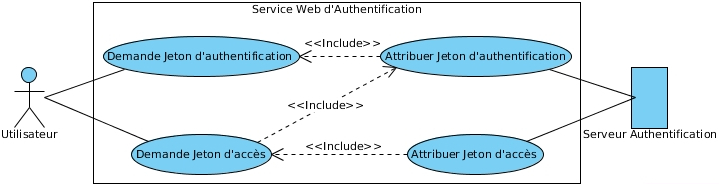
\includegraphics[width=.9\textwidth]{sprint3-webservices-oauth-usecase}
    \caption{Diagramme de case d'utilisation d'authentification --- Itération 3}
\label{fig:sprint3-webservices-oauth-usecase}
\end{figure}

La figure~\ref{fig:sprint3-webservices-oauth-sequence} présente le diagramme de
séquence du service d'authentification.

\begin{figure}[H]
    \centering
    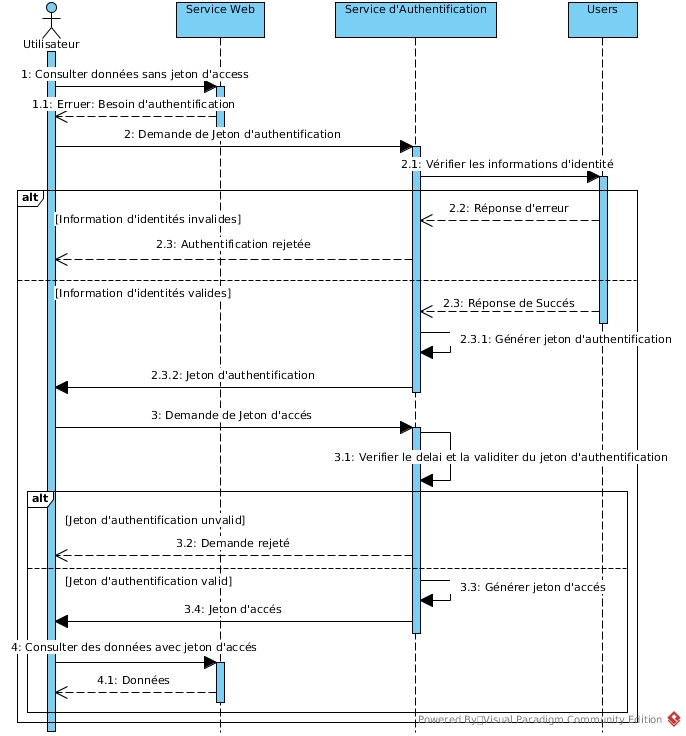
\includegraphics[width=1\textwidth]{sprint3-webservices-oauth-sequence}
    \caption{Diagramme de séquence d'authentification --- Itération 3}
\label{fig:sprint3-webservices-oauth-sequence}
\end{figure}

La figure~\ref{fig:sprint3-dashboard-classs} décrit le diagramme des classes du
page \textquote{Dashboard} dans la troisième itération.

\begin{figure}[H]
    \centering
    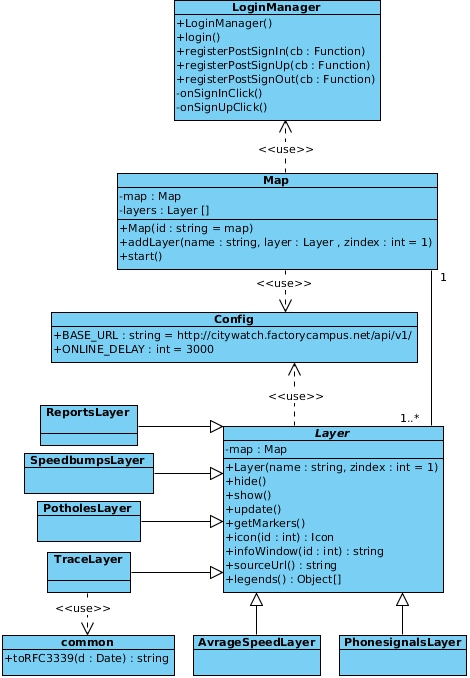
\includegraphics[width=.8\textwidth]{sprint3-dashboard-class}
    \caption{Diagramme des classes du Dashboard --- Itération 3}
\label{fig:sprint3-dashboard-classs}
\end{figure}

La figure~\ref{fig:sprint3-webservices-class} présente le diagramme de classes
du service web de la troisième itération.

\begin{figure}[H]
    \centering
    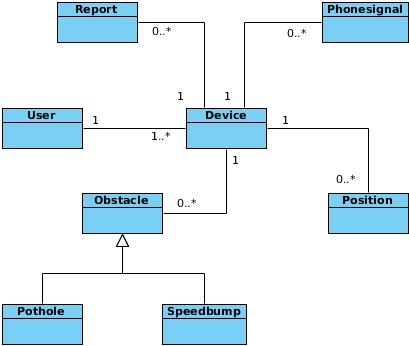
\includegraphics[width=0.9\textwidth]{sprint3-webservices-class}
    \caption{Diagramme de classe du services web --- Itération 3}
\label{fig:sprint3-webservices-class}
\end{figure}

Le schéma de la base de données de cette itération est dans
l'annexe~\ref{sec:sprint3-database}.

\section{Revue de cette itération}

% On rappelons que nous travaillons dans un équipe Scrum qui nécessite
% l'intégration de notre travail dans le projet pour attendre le but.

\subsection{Produit de l'itération}

\subsubsection{Légende du Dashboard}

Dans cette page nous travaillons sur deux parties:

\begin{itemize}
    \item la première: active/désactive les boutons de filtrage de chaque
        marqueur.
    \item la deuxième: gérer la communication interne entre serveur et la page.
\end{itemize}

Aussi, nous participons 80\% à l'ajout de légende à notre carte et affiche le
filtrage des marqueurs.

\begin{figure}[H]
\centering
    \begin{subfigure}{.7\textwidth}
    \centering
  \centering
  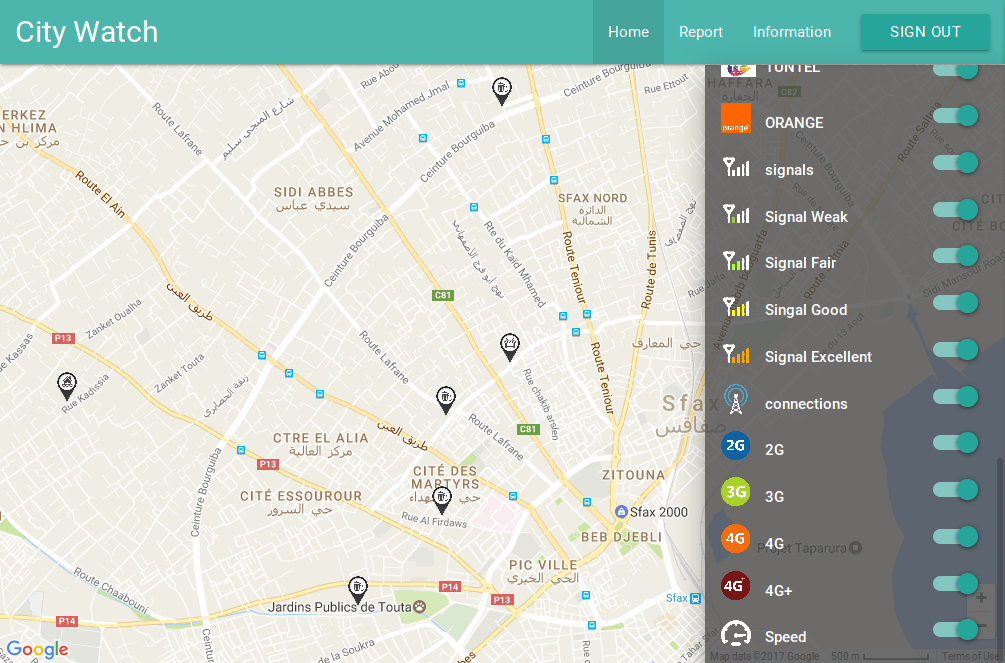
\includegraphics[width=\linewidth, height=5.5cm]{sprint3-dashboard-screenshot1}
  \caption{Marqueurs activés}
\label{fig:sprint3-dashboard-screenshot1}
\end{subfigure}
\begin{subfigure}{.7\textwidth}
    \centering
  \centering
  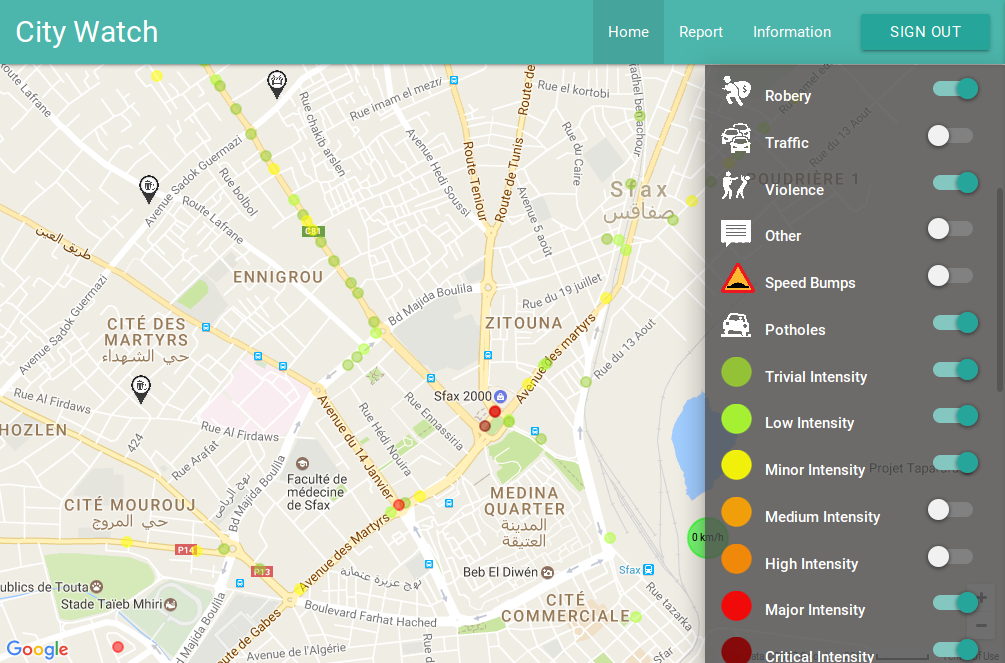
\includegraphics[width=\linewidth, height=5.5cm]{sprint3-dashboard-screenshot2}
  \caption{Quelques marqueurs désactivés}
\label{sprint3-dashboard-screenshot2}
\end{subfigure}
\caption{Dashboard \textquote{City Watch} à la troisième itération}
\end{figure}

\subsubsection{Android}

Les données captées par l'application mobile (Position, Secousses,
Ralentisseur, Réseaux, force du signal et vitesse) sont récupérées par le
serveur pour assurer la sauvegarde et la transmission vers une base données.

\begin{figure}[H]
\centering
    \begin{subfigure}{.4\textwidth}
    \centering
  \centering
  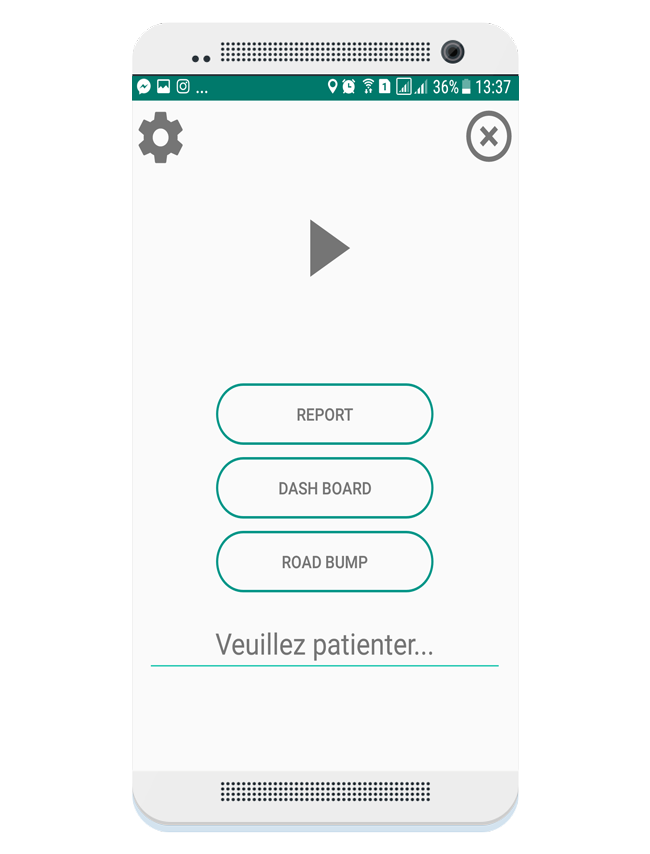
\includegraphics[width=1.0\linewidth]{sprint3-android-screenshot1}
  \caption{État désactivé}
\label{fig:sprint3-android-screenshot1}
\end{subfigure}
\begin{subfigure}{.4\textwidth}
    \centering
  \centering
  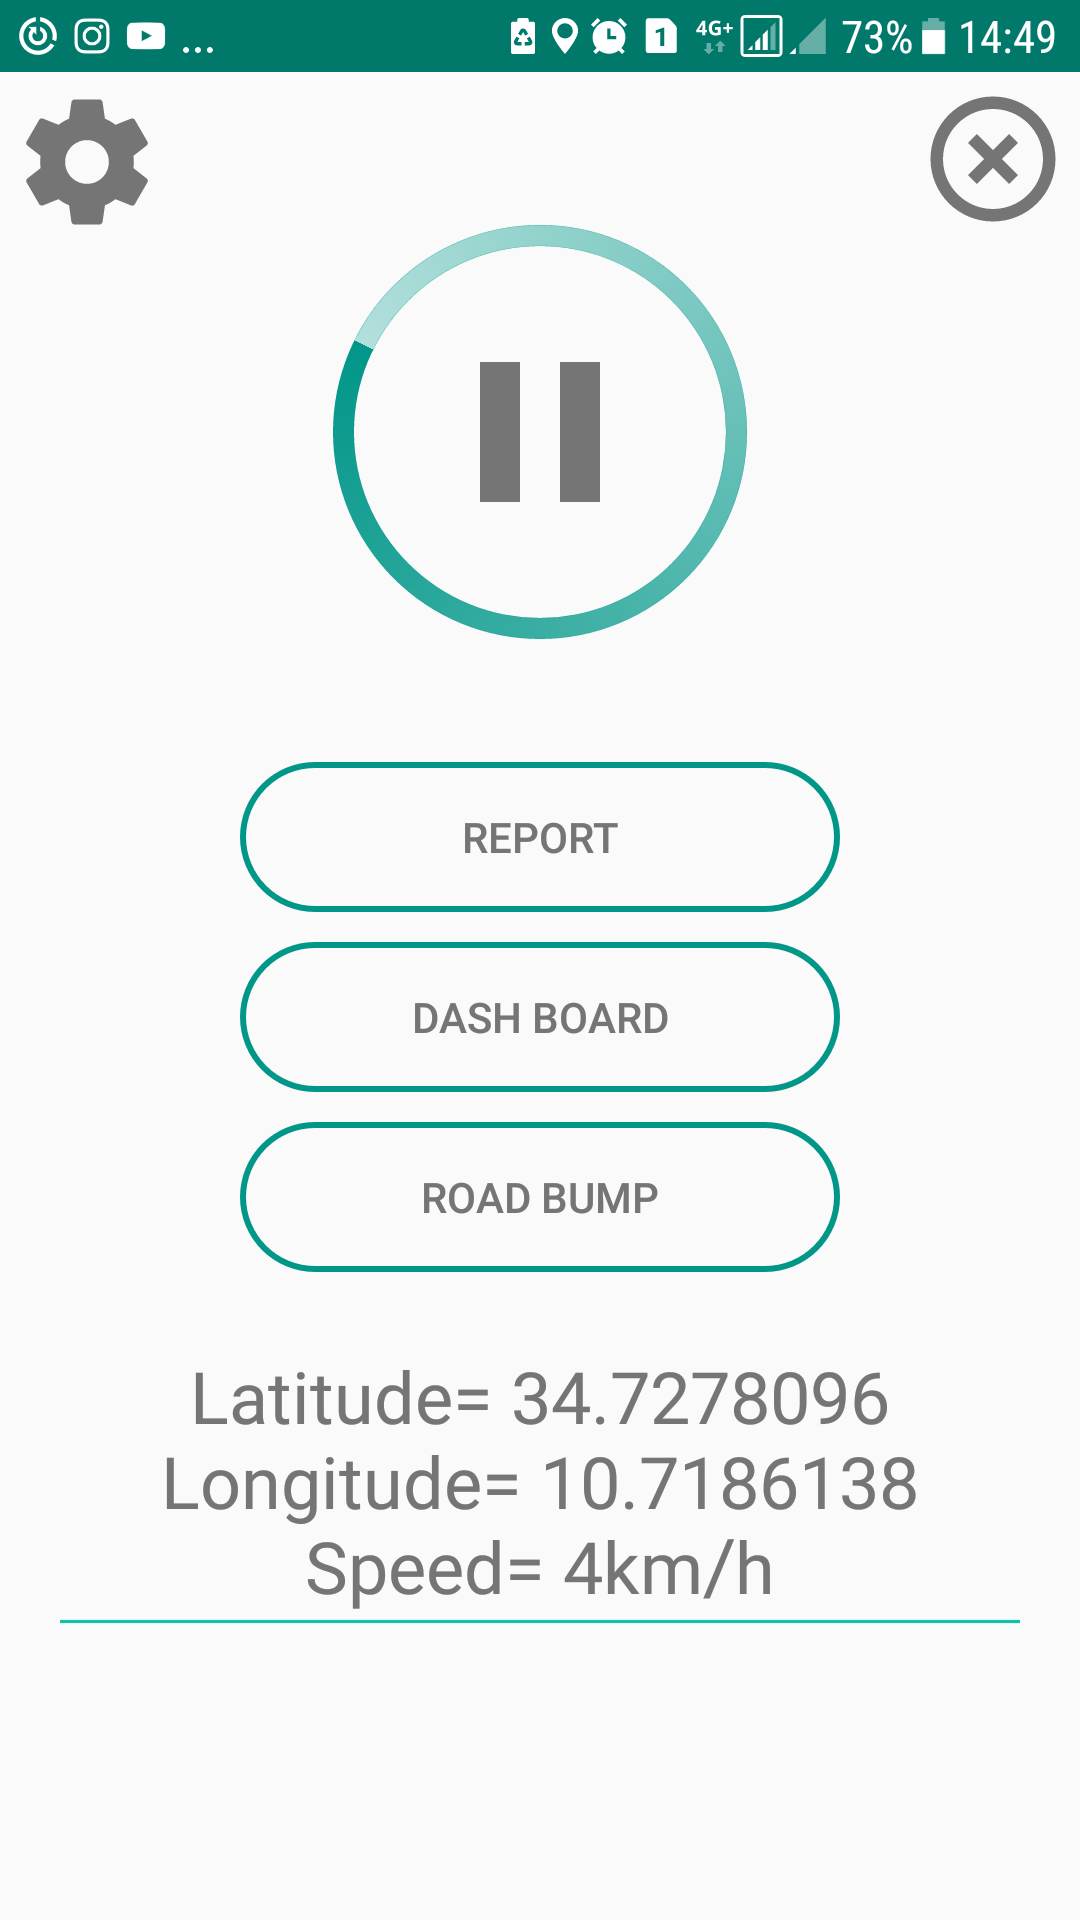
\includegraphics[width=1.0\linewidth]{sprint3-android-screenshot2}
  \caption{État activé}
\label{fig:sprint3-android-screenshot2}
\end{subfigure}
\caption{Interface de l'application à la troisième itération}
\end{figure}

\subsection{Avis du Product Owner}

Après la présentation du produit final, le \textquote{Product Owner} était très
satisfait a notre travail.

\subsection{Burndown chart}

La figure~\ref{fig:sprint3-burndown} présente une vue d'ensemble sur le progrès
de notre travail au cours de l'itération par rapport au progrès idéal.

\usetikzlibrary{plotmarks}

\begin{figure}
\centering
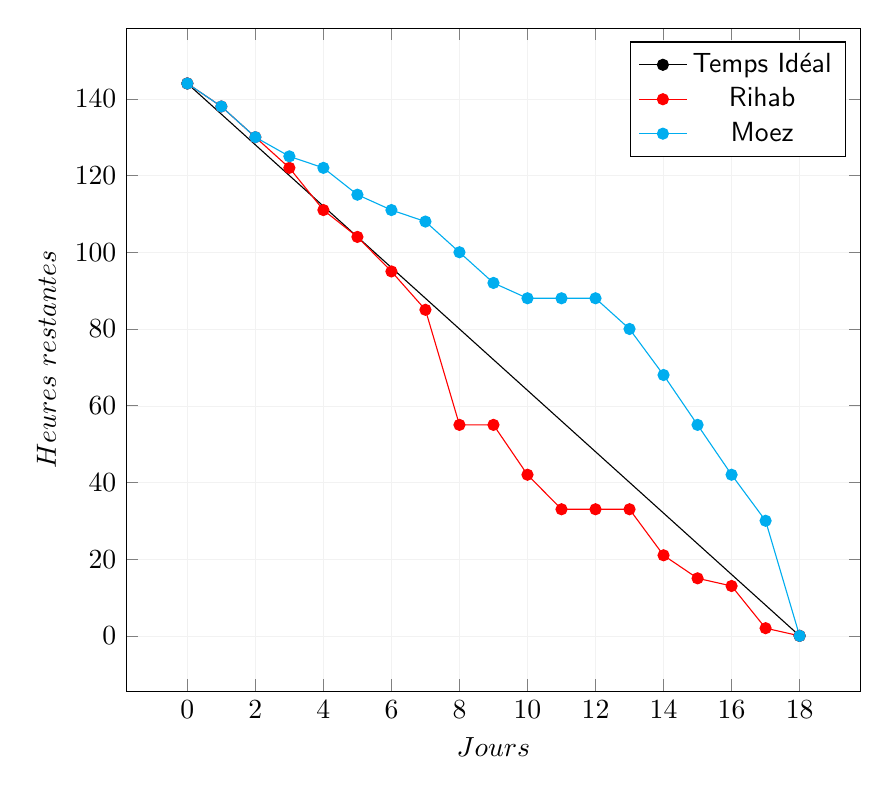
\begin{tikzpicture}[y=.2cm, x=.7cm,font=\sffamily]
\begin{axis}[
xlabel=$Jours$,
ylabel=$Heures\ restantes$,
grid=both,
grid style={line width=.1pt, draw=gray!10},
width=0.9\textwidth,
height=10cm,
%major grid style={line width=.2pt,draw=gray!50},
]
\addplot[color=black,mark=*] coordinates {
        (0,144)
        (18,0)
    };
    \addlegendentry{Temps Idéal}

    \addplot[mark=*,red] plot coordinates {
        (0, 144)
        (1, 138)
        (2, 130)
        (3, 122)
        (4, 111)
        (5, 104)
        (6, 95)
        (7, 85)
        (8, 55)
        (9, 55)
        (10, 42)
        (11, 33)
        (12, 33)
        (13, 33)
        (14, 21)
        (15, 15)
        (16, 13)
        (17, 2)
        (18, 0)
       
    };
    \addlegendentry{Rihab}
      \addplot[mark=*,cyan] plot coordinates {
       (0, 144)
        (1, 138)
        (2, 130)
        (3, 125)
        (4, 122)
        (5, 115)
        (6, 111)
        (7, 108)
        (8, 100)
        (9, 92)
        (10, 88)
        (11, 88)
        (12, 88)
        (13, 80)
        (14, 68)
        (15, 55)
        (16, 42)
        (17, 30)
        (18, 0)
       
    };
    \addlegendentry{Moez}
\end{axis}
\end{tikzpicture}
\caption{Graphique d'avancement - Itération 3}
\end{figure}


Le tableau~\ref{tab:sprint3-evaluation} présente le pourcentage de réalisation
de nos tâches de cette itération.

\begin{center}
    \begin{longtable}{| l | l |}
        \caption{Liste des tâches réalisées de la troisième itération}
\label{tab:sprint3-evaluation} \\

        \hline
        \textbf{Les tâches} & \textbf{Taux de réalisation} \\ \hline
        \endhead

        \hline \multicolumn{2}{|r|}{{Continué en page suivante$\dotsc$}} \\ \hline
        \endfoot

        \hline \hline
        \endlastfoot

        \hline
Intégration Dashboard et Rapport dans l'application Android & Effectué 100\% \\ \hline
Authentification RESTful & Effectué 100\% \\ \hline
Landing page & Effectué 100\% \\ \hline
Compte utilisateur & Effectué 100\% \\ \hline
Service d’enregistrement les informations du réseau & Effectué 100\% \\ \hline
Service de récupération des informations réseaux & Effectué 100\% \\ \hline
Service d’enregistrement de la vitesse du véhicule & Effectué 100\% \\ \hline
Service de récupération de la vitesse & Effectué 100\% \\ \hline
Application Android Responsive & Effectué 100\% \\ \hline
Recherche Business intelligence & Effectué 100\% \\ \hline
Intégrer la base de données avec BI & Effectué 30\% \\ \hline
Logo du \textquote{City Watch} & Effectué 80\% \\ \hline
Étude scénario de commercial d’embouteillage & Effectué 100\% \\ \hline
Rectification du service de chargement d’image & Effectué 100\% \\ \hline
Étude scénario de commercial des secousses & Effectué 100\% \\ \hline
\end{longtable}
\end{center}

\section*{Conclusion}
\addcontentsline{toc}{section}{Conclusion}

A fin de cette itération, nous avons découvert des nouveaux aspects
intéressants dans notre projet qui nécessitent l'intervention des technologies
(Big Data, Data mining, \ldots).
